\PassOptionsToPackage{svgnames}{xcolor}
\documentclass[12pt]{article}

%\usepackage{etex}

\usepackage[T1]{fontenc}
%\usepackage{textcomp}
\renewcommand{\rmdefault}{ptm} % Load in the Times font
%\usepackage[scaled=0.94]{helvet}
\usepackage[subscriptcorrection,slantedGreek,nofontinfo,mtpcal]{mtpro2}
\let\Bbbk\relax
\usepackage[use-ref]{exSheets}
\usepackage{xcolor}
%\usepackage{tcolorbox, needspace}
\usepackage[top=1in, bottom=1in, left=1in, right=1in]{geometry}
%\usepackage[some]{background}
\usepackage{epigraph}

%\usepackage{sectsty}
\usepackage{amsmath}
\usepackage{amsfonts}
\usepackage{amssymb}
\usepackage{graphics}
\usepackage{caption}
\usepackage{kbordermatrix}
\usepackage{float}
\usepackage{cprotect}
\usepackage{ifthen}

\usepackage{enumerate}
%\usepackage{enumitem}

\newcommand{\bgamma}{\mbox{\boldmath $\Gamma$}}

\newcommand{\bOne}{\textbf{1}}
\newcommand{\bphi}{\mbox{\boldmath $\phi$}}
\newcommand{\bPhi}{\mbox{\boldmath $\Phi$}}

\newcommand{\Km}{\text{K}_\text{m}}
\newcommand{\Vm}{\text{V}_\text{m}}

\newcommand{\bA}{\mbox{\boldmath $A$}}
\newcommand{\bB}{\mbox{\boldmath $B$}}
\newcommand{\bC}{\mbox{\boldmath $C$}}
\newcommand{\bD}{\mbox{\boldmath $D$}}
\newcommand{\bF}{\mbox{\boldmath $F$}}
\newcommand{\bH}{\mbox{\boldmath $H$}}
\newcommand{\bL}{\mbox{\boldmath $L$}}
\newcommand{\bT}{\mbox{\boldmath $T$}}
\newcommand{\bI}{\mbox{\boldmath $I$}}
\newcommand{\bM}{\mbox{\boldmath $M$}}
\newcommand{\bN}{\mbf{N}}
\newcommand{\bQ}{\mbox{\boldmath $Q$}}
\newcommand{\bP}{\mbox{\boldmath $P$}}
\newcommand{\bR}{\mbox{\boldmath $R$}}
\newcommand{\bX}{\mbox{\boldmath $X$}}
\newcommand{\bY}{\mbox{\boldmath $Y$}}
\newcommand{\bU}{\mbox{\boldmath $U$}}
\newcommand{\bV}{\mbox{\boldmath $V$}}

\newcommand{\bx}{\mbox{\boldmath $x$}}
\newcommand{\bb}{\mbox{\boldmath $b$}}
\newcommand{\bc}{\mbox{\boldmath $c$}}
\newcommand{\bg}{\mbox{\boldmath $g$}}
\newcommand{\bff}{\mbox{\boldmath $f$}}
\newcommand{\bn}{\mbox{\boldmath $n$}}
\newcommand{\bv}{\mbox{\boldmath $v$}}
\newcommand{\bu}{\mbox{\boldmath $u$}}
\newcommand{\bJ}{\mbox{\boldmath $J$}}
\newcommand{\bZero}{\mbox{\boldmath $0$}}
\newcommand{\bLo}{\mbox{\boldmath $L_0$}}
\newcommand{\bNo}{\mbox{\boldmath $N_0$}}
\newcommand{\bNr}{\mbox{\boldmath $N_R$}}
\newcommand{\bNIC}{\mbox{\boldmath $N_{IC}$}}
\newcommand{\bNDC}{\mbox{\boldmath $N_{DC}$}}
\newcommand{\bJM}{\mbox{\boldmath $J_M$}}
\newcommand{\bJC}{\mbox{\boldmath $J_C$}}
\newcommand{\bK}{\mbox{\boldmath $K$}}
\newcommand{\bKo}{\mbox{\boldmath $K_0$}}
\newcommand{\bS}{\mbf{S}}
\newcommand{\bs}{\mbf{s}}
\newcommand{\bSi}{\mbox{\boldmath $S_i$}}
\newcommand{\bSd}{\mbox{\boldmath $S_d$}}
\newcommand{\bdSi}{\mbox{\boldmath $d\!S_i$}}
\newcommand{\bdSd}{\mbox{\boldmath $d\!S_d$}}
\newcommand{\bdS}{\mbf{dS}}
\newcommand{\bdx}{\mbox{\boldmath $dx$}}
\newcommand{\dt}{d\!t}
\newcommand{\bdt}{\mbox{\boldmath $dt$}}
%\newcommand{\bdSdt}{\mbox{$\displaystyle \frac{\bdS}{\bdt}$}}
\newcommand{\bdSdt}{\frac{d\!\bs}{\dt}}
\newcommand{\bdxdt}{\frac{d\bvx}{\dt}}
\newcommand{\el}[2]{\varepsilon^{#1}_{#2}}
\newcommand{\bdSddt}{\mbox{$\displaystyle \frac{\bdS_d}{\bdt}$}}
\newcommand{\bdSidt}{\mbox{$\displaystyle \frac{\bdS_i}{\bdt}$}}
\newcommand{\bp}{\mbox{\boldmath $p$}}
\newcommand{\dA}{d\!A}
\newcommand{\dB}{d\!B}
\newcommand{\dX}{d\!X}
\newcommand{\dY}{d\!Y}
\newcommand{\dZ}{d\!Z}
\newcommand{\dP}{d\!P}
\newcommand{\dQ}{d\!Q}
\newcommand{\dS}{d\!S}
\newcommand{\ESI}{E\!S\!I}
\newcommand{\ES}{E\!S}
\newcommand{\dy}{d\!y}
\newcommand{\dx}{d\!x}
\newcommand{\du}{d\!u}
\newcommand{\dv}{d\!v}
\newcommand{\df}{d\!f}

\newcommand{\bvp}{\textbf{p}}
\newcommand{\bvx}{\textbf{x}}
\newcommand{\bvf}{\textbf{f}}
\newcommand{\bvm}{\textbf{m}}
\newcommand{\bvv}{\textbf{v}}
\newcommand{\bvu}{\textbf{u}}
\newcommand{\bvy}{\textbf{y}}
\newcommand{\bvs}{\textbf{s}}

\newcommand{\bds}{\mbox{\boldmath $ds$}}
\newcommand{\ratev}{\mbox{\boldmath $v$}}
\newcommand{\bdsdt}{\frac{\bds}{\bdt}}

\newcounter{innerlist}
\renewcommand{\theinnerlist}{\alph{innerlist}.}
\newcommand{\inneritem}[1]{\refstepcounter{innerlist}\theinnerlist\quad #1}


\usepackage{tikz}
\usepackage[object=vectorian]{pgfornament} %%  http://altermundus.com/pages/tkz/ornament/index.html
\usetikzlibrary{calligraphy}
\usetikzlibrary{arrows, arrows.meta,plotmarks}
\usetikzlibrary{matrix}

% Rounded end arrows
\tikzset{
    regulations/.cd,
    act/.style={-{Circle}}, % Style for activation
    rep/.style={-{Bar}}, % Style for repression
}
\newcommand{\regulationarrow}[1][act]{%
    \tikz[baseline] {\draw[thick,regulations/#1] (0,0.5ex) --++ (1.5em,0);}%
}


\parindent=0pt

\DeclareInstance{exsheets-heading}{fancy}{default}{
 toc-reversed = true,
 indent-first = true,
 vscale = 2 ,
 %pre-code = \rule{\linewidth}{1pt} ,
 %post-code = \rule{\linewidth}{1pt} ,
 title-format = \large\scshape\color{FireBrick},
 number-format = \large\bfseries\color{black},
 points-format = \itshape,
 join = { number[r,B]title[l,B](1ex,0pt) },
 attach =
 {
 main[hc,vc]number[hc,vc](0pt,0pt) ;
 main[l,vc]points[r,vc](-\marginparsep,0pt)
 }
 }


\DeclareInstance{exsheets-heading}{simple}{default}
{
 %runin=true,
 %above = \parskip ,
 below = 6pt,
 title-format = \normalsize,
 points-pre-code = ( ,
 points-post-code = ) ,
 title-format = \large\scshape\color{FireBrick},
 number-format = \large\bfseries\color{black},
 attach = { main[l,t]number[l,t](0pt,0pt) },
 %attach = { main[l,t]number[l,t](0pt,0pt) } ,
 join =
  {
  number[r,b]title[l,b](1ex,0pt) ;
  main[l,b]points[l,t](1em,0pt)
  }
}


\SetupExSheets{
    headings=simple,
    skip-below=1em,
    question/type=exercise
    }


% Set this flag to determine whether to print the solutions or not
% -------------------------------------------------------------------
\newboolean{myPrintSolutions}
\setboolean{myPrintSolutions}{true}
% -------------------------------------------------------------------

\renewcommand\epigraphflush{flushleft}
\renewcommand\epigraphsize{\normalsize}
\setlength\epigraphwidth{0.7\textwidth}

\definecolor{titlepagecolor}{cmyk}{1,.60,0,.40}

\DeclareFixedFont{\titlefont}{T1}{ppl}{b}{it}{0.5in}

\makeatletter
\def\printauthor{%
    {\large \@author}}
\makeatother
\author{%
    Herbert M Sauro \\
    Bioengineering \\
    \texttt{hsauro@uw.edu}\vspace{20pt}
    }


% Taken from https://tex.stackexchange.com/questions/85904/showcase-of-beautiful-title-page-done-in-tex
\newcommand\titlepagedecoration{%
\begin{tikzpicture}[remember picture,overlay,shorten >= -10pt]

\coordinate (aux1) at ([yshift=-15pt]current page.north east);
\coordinate (aux2) at ([yshift=-410pt]current page.north east);
\coordinate (aux3) at ([xshift=-5.5cm]current page.north east);
\coordinate (aux4) at ([yshift=-150pt]current page.north east);

\begin{scope}[titlepagecolor!40,line width=12pt,rounded corners=12pt]
\draw
  (aux1) -- coordinate (a)
  ++(225:5) --
  ++(-45:5.1) coordinate (b);
\draw[shorten <= -10pt]
  (aux3) --
  (a) --
  (aux1);
\draw[opacity=0.6,titlepagecolor,shorten <= -10pt]
  (b) --
  ++(225:2.2) --
  ++(-45:2.2);
\end{scope}
\draw[titlepagecolor,line width=8pt,rounded corners=8pt,shorten <= -10pt]
  (aux4) --
  ++(225:0.8) --
  ++(-45:0.8);
\begin{scope}[titlepagecolor!70,line width=6pt,rounded corners=8pt]
\draw[shorten <= -10pt]
  (aux2) --
  ++(225:3) coordinate[pos=0.45] (c) --
  ++(-45:3.1);
\draw
  (aux2) --
  (c) --
  ++(135:2.5) --
  ++(45:2.5) --
  ++(-45:2.5) coordinate[pos=0.3] (d);
\draw
  (d) -- +(45:1);
\end{scope}
\end{tikzpicture}%
}


\begin{document}

\begin{titlepage}

\noindent
\titlefont Systems Biology Exercises\par
\epigraph{What is the difference between a live cat and a dead cat?  A dead cat is a collection of its component parts. A live cat is the emergent behavior of the systems incorporating those parts. In pursuit of systems. Nature 435, 1 (2005). }%
{\textit{London 2005}\\ \textsc{Anonymous}}
\null\vfill
\vspace*{1cm}
\noindent
\hfill
\begin{minipage}{0.35\linewidth}
    \begin{flushright}
        \printauthor
    \end{flushright}
\end{minipage}
%
\begin{minipage}{0.02\linewidth}
    \rule{1pt}{125pt}
\end{minipage}
\titlepagedecoration
\end{titlepage}

%\sectionlinetwo{DarkGreen}{88}

\begin{center}
{\huge\bf Exercises and Solutions for\\[-2pt] Modeling Systems Biology:\\[5pt] Introduction to Pathway Modeling}\\[8pt]
{\bf\Large 2021, v1.0}
\end{center}

August, 30, 2021

\begin{center}

\begin{tikzpicture}[line width=2pt]
\node[minimum size=0.1cm]{};
\pen (0,0);
\calligraphy (-7,0) -- (8,0);
%\fill (-1,-.25) -- ++(1,.1mm) -- ++(1,-.1mm) -- ++(-1,-.1mm) -- cycle;
%\fill (0,-0.5) circle[x radius=1cm, y radius=.1mm];
\end{tikzpicture}
\end{center}

% ---------------------------------------------------------------------------------------------
\section{Biology}
% ---------------------------------------------------------------------------------------------

In the following exercises use the data given in the main text along with Tables 1.3, 1.4, 1.5 and 1.6 of the textbook.
\medskip

\begin{question}
How many {\em E.\ coli} cells laid end to end would fit across the full stop at the end of this sentence? Assume the diameter of the full stop is 0.5 mm.
\end{question}
\begin{solution}
Assuming the length of cell is 2$\mu m$ the answer will be 250 cells.
\end{solution}


\begin{question}
Estimate the volume of an {\em E.\ coli} cell.
\end{question}
\begin{solution}
Assume {\em E.\ coli} is a cylinder: volume = $1.57 \mu m^3$ or $1.57 \times 10^{-15}$ L
\end{solution}


\begin{question}
\begin{enumerate}[a)]
\item Calculate the surface area of an {\em E.\ coli} cell assuming its a cylinder.

\item If a typical membrane protein is 5 nm in diameter, estimate the number of membrane proteins that can be laid out on the membrane if the center-center distance between each protein is 6 nm.
\end{enumerate}
\end{question}
\begin{solution}
\begin{enumerate}[a)]
\item Assume {\em E.\ coli} is a cylinder: Area = 7.85 $\mu m^2$
\item Approximately 218,000 proteins
\end{enumerate}
\end{solution}


\begin{question}
Show that a 1 nM concentration is roughly equivalent to 1 molecule in a volume of 1 {\em E.\ coli} cell.
\end{question}
\begin{solution}
The volume of an {\em E.\ coli} cell is approximately $1.5 \times 10^{-15}$ L. 1 nM represents approximately $10^{-9} \times 1.5 \times 10^{-15}$ moles in a cell. Multiply by avogadro's number to get the number of molecules: $6 \times 10^{23} = 0.9$. This is roughly one molecule per {\em E.\ coli} cell.
\end{solution}


\begin{question}
Estimate the number of protein molecules a typical {\em E.\ coli} cell can make per second assuming the average protein is 360 amino acids long. Assume that the number of proteins in a cell is 3,000,000. How long would it take to make 3,000,000 proteins? % 2000 proteins per second, assume, 18000 ribosomes and 40 aa/sec
\end{question}
\begin{solution}
 25 minutes (1500 seconds)
\end{solution}


\begin{question}
If it takes 1,500 ATP molecules to make an average protein, how long would it take before all the ATP is used up? Assume the ATP is not being replaced. % 2000 proteins per sec, 3000000 ATP per sec, Ans 1:
\end{question}
\begin{solution}
0.67 seconds
\end{solution}


\begin{question}
E.\ coli can be considered a cylindrical volume with length $2\ \mu m$ and diameter $1\ \mu m$. A reaction is known to occur in {\em E.\ coli} with an intensive rate of $0.5\ \mbox{mmol } s^{-1}\ l^{-1}$.
\begin{enumerate}[a)]
\item What is the rate of reaction per volume of {\em E.\ coli}?
\item If Avogadro's number is $6.022 \times 10^{23}$, express the rate in terms of molecules converted per second per {\em E.\ coli}.
\end{enumerate}
\end{question}
\begin{solution}
\begin{enumerate}[a)]
\item $5 \times 10^{-16}$ mmoles per second per volume of {\em E.\ coli}

\item $3 \times 10^{5}$ per second per {\em E.\ coli}
\end{enumerate}
\end{solution}


\begin{question}
What are the visual symbols often used to represent activation and repression in biochemical networks?
\end{question}
\begin{solution}
Repression or inhibition is often depicted using a blunt end: $A\ \raisebox{-.2ex}{\rotatebox{90}{\scalebox{1}[1.2]{$\bot$}}}\ B$ where as activation often uses a simple arrow $A \rightarrow B$ or a filled circle end:
$A\ \regulationarrow[act]\ B$.
\end{solution}


\begin{question}
Draw a similar diagram to the glycolysis regulatory diagram (Figure 1.4) but for the lysine, threonine and methionine biosynthesis pathway from {\em E.\ coli}.
\end{question}
\begin{solution}
Research amino acid biosynthesis pathways online. You will discover that these pathways have a number of negative feedback loops that go form the end product to the start of the pathway. You may also notice that there are nested feedback loops.
\end{solution}


\begin{question}
Why is the size of an organism's genome a poor indicator of the organism's complexity?
\end{question}
\begin{solution}
Many expressed proteins are covalently modified or form complexes. This is particularly the case for mammalian systems where covalent modifications is endemic amount proteins. This means that the number of states far exceeds the number of gene encoded on a genome.
\end{solution}


\begin{question}
Describe the basic approach used to find network motifs.
\end{question}
\begin{solution}
See page section 1.8 of the textbook
\end{solution}


\begin{question}
Looking at motif c) in Figure 1.23 in the textbook, try to explain how it might operate as a memory unit.
\end{question}
\begin{solution}
The two inhibitory arcs around the two lower nodes ensurers that only one can be active at anyone time. The $z$ node can be used to flip that state to the other node. For example, if the right-hand node is active then the left-hand node will be inactive. If $z$ is brought to a high value, this will inhibit the right-node and activate the left-node thus changing the state. If the $z$ node is now brought low, the state of the two nodes remains unchanged. In this sense the network has recorded the $z$ event and thus acts as a memory unit.
\end{solution}


\begin{question}
Study the network shown below and try to figure out its function. Use Figures 1.22, 1.23, and 1.24 in the textbook as guides.

\begin{center}
  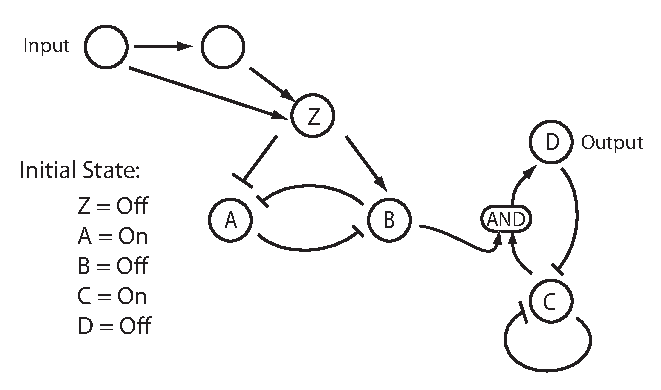
\includegraphics[scale = 0.8]{ComplicatedMotif}
\end{center}

The AND block on the left of the network represents an AND gate, that is the output of the block is only active if {\em both} inputs are also active.
\end{question}
\begin{solution}
The first part of the network is a noise filter so that node $z$ is only active when the input has a sufficiently long duration. When $z$ rises it flips the state of nodes $A$ and $B$ so that $B$ becomes active. Note that when the input signal returns to its quiescent state, the state of $B$ remains high because of the two inhibitory arcs between $A$ and $B$. With $B$ active, it turns on the output $D$ via the AND gate. This last motif is a relaxation oscillator and and as result it will start to oscillate. The `function' of the entire network is to detect a signal on the input and use that signal to permanently activate an oscillator.
\end{solution}


\ifthenelse{\boolean{myPrintSolutions}}{
\medskip
\begin{center}
{\bf\large Solutions}
\end{center}

\printsolutions[section]
}{}

% ---------------------------------------------------------------------------------------------
\section{Kinetics}
% ---------------------------------------------------------------------------------------------

\begin{question}
Define the following terms:
\begin{enumerate}[a)]
  \item Stoichiometric amount
  \item Stoichiometric coefficient
  \item Rate of change
  \item Rate of reaction
\end{enumerate}
\end{question}
\begin{solution}
\begin{enumerate}

\item The stoichiometric amount is the number of molecules a particular reactant or product
takes part in a given reaction

\item $c_i = $ molar amount of product - molar amount of reactant. In reactions where the species only appears on the reactant side, the stoichiometric coefficient is the negative of the stoichiometric amount of the reactant. In reactions where the species only appears on the product side, the stoichiometric coefficient is the stoichiometric amount of the product.

\item The rate of change is defined as the rate of change in concentration or amount of a designated molecular species.

\item The rate of reaction is the rate of change of a given species normalized by its stoichiometric coefficient.

\end{enumerate}
\end{solution}

\begin{question}
What are the stoichiometric amounts and stoichiometric coefficients for each species in the following reactions:
%
\begin{align*}
 \text{A} &\longrightarrow \text{B} \\
 \text{A} + \text{B} &\longrightarrow \text{C} \\
 \text{A} &\longrightarrow \text{B} + \text{C} \\
 2 \text{A} &\longrightarrow \text{B} \\
 3 \text{A} + 4 \text{B} &\longrightarrow 2 \text{C} + \text{D} \\
 \text{A} + \text{B} &\longrightarrow \text{A} + \text{C} \\
 \text{A} + 2 \text{B} &\longrightarrow 3 \text{B} + \text{C} \\
\end{align*}
\end{question}
\begin{solution}
\begin{enumerate}
  \item 1, 1; -1, 1
  \item 1, 1, 1; -1, -1, 1
  \item 1, 1, 1; -1, 1, 1
  \item 2, 1; -2, 1
  \item 3, 4, 2, 1; -3, -3, 2, 1
  \item 1, 1, 1, 1; 0, -1, 1
  \item 1, 2, 3, 1; -1, 1, 1
\end{enumerate}
\end{solution}

\begin{question}
Write out the mass-action rate laws for the following elementary reactions:
\begin{enumerate}[a)]
  \item $ A \rightarrow $
  \item $ A + B \rightarrow $
  \item $A + 2 B \rightarrow $
  \item $2 A \rightarrow $
\end{enumerate}
\end{question}
\begin{solution}
\begin{enumerate}[a)]
  \item $ v = k A $
  \item $ v = k A B $
  \item $v = k A B^2 $
  \item $v = k A^2 $
\end{enumerate}
\end{solution}

\begin{question}
Write out the reversible mass-action rate laws for the following reactions:
\begin{enumerate}
  \item $ A \rightarrow B $
  \item $ A + B \rightarrow C + D $
  \item $2 A + B \rightarrow 2 C $
  \item $A \rightarrow 2 B $
\end{enumerate}
\end{question}

\begin{solution}
a) $k_1 A - k_2 B$; \ b) $k_1 A B$ - k_2 C D; \ c) $k_1 A^2 B - k_2 C^2$; \ d) $k_1 A^2 - k_2 B^2$
\end{solution}

\begin{question}
A reversible reaction $A \rightleftharpoons B$ has an equilibrium constant of 5.0. If at equilibrium the concentration of $A$ is 2 mM, what is the equilibrium concentration of $B$?
\end{question}

\begin{solution}
Since $K_{eq} = B/A = 5$, and $A = 2$, therefore $B = A \times K_{eq} = 10$ mM
\end{solution}


\begin{question}
Define the following terms:

\begin{enumerate}[a)]
  \item Mass-action ratio
  \item Disequilibrium ratio
\end{enumerate}
\end{question}

\begin{solution}
\begin{enumerate}[a)]
\item The mass-action ratio, $\Gamma$, is the ratio of products to the reactants {\em in vivo}. At equilibrium $\Gamma = K_{eq}$.
\item The disequilibrium ratio, $\rho$, is the ratio of the mass-action ratio and equilibrium constant.
\end{enumerate}
\end{solution}

\ifthenelse{\boolean{myPrintSolutions}}{
\medskip
\begin{center}
{\bf\large Solutions}
\end{center}

\printsolutions[section]
}{}

% ---------------------------------------------------------------------------------------------
\section{Networks}
% ---------------------------------------------------------------------------------------------


\begin{question}
Derive a set of differential equations for the following model in terms of the
rate of reaction, $v_1$, $v_2$, and $v_3$:
%%
\begin{align*}
  \text{A} &\stackrel{v_1}{\rightarrow} 2 \text{B} \\
  \text{B} &\stackrel{v_2}{\rightarrow} 2 \text{C} \\
  \text{C} &\stackrel{v_3}{\rightarrow} \emptyset
\end{align*}
\end{question}
\begin{solution}
$$\frac{dA}{dt} =  -v_1;\ \quad \frac{dB}{dt} = 2 v_1 - v_2;\ \quad \frac{dC}{dt} = 2 v_2 - v_3 $$
\end{solution}


\begin{question}
Derive the stoichiometry matrix for the previous model.
\end{question}
\begin{solution}
\begin{equation*}
         \left[ \begin{array}{rrrr}
           -1 &  0 &  0 \\
            2 & -1 &  0 \\
            0 &  2 & -1 \\
         \end{array} \right]
\end{equation*}
\end{solution}


\begin{question}
Derive the set of differential equations for the following model in terms of the
rate of reaction, $v_1$, $v_2$ and $v_3$:
%
\begin{align*}
  \text{A} &\stackrel{v_1}{\rightarrow} \text{B} \\
  2 \text{B} + \text{C} &\stackrel{v_2}{\rightarrow} \text{B} + \text{D} \\
  \text{D} &\stackrel{v_3}{\rightarrow} \text{C} + \text{A}
\end{align*}
\end{question}
\begin{solution}
$$ \frac{dA}{dt} =  v_3 - v_1;\ \quad \frac{dB}{dt} = v_1 - 2 v_2 + v_2 = v_1 - v_2 $$

$$ \frac{dC}{dt} = v_3 - v_2;\ \quad \frac{dD}{dt} = v_2 - v_3 $$
\end{solution}

\begin{question}
Derive the stoichiometry matrix for the previous model.
\end{question}
\begin{solution}
\begin{equation*}
         \left[ \begin{array}{rrrr}
           -1 &  0 &  1  \\
            1 & -1 &  0  \\
            0 & -1 &  1  \\
            0 &  1 & -1  \\
         \end{array} \right]
\end{equation*}
\end{solution}


\begin{question}
Enter the previous models, 3 and 4, into Tellurium and confirm that the stoichiometry matrices are the same as those derived manually in the previous question.
\end{question}
\cprotEnv\begin{solution}
\begin{enumerate}[a)]
\item
\begin{verbatim}
import tellurium as te

r = te.loada('''
   A -> 2B; v1;
   B -> 2C; v2;
   C ->; v3
   v1 = 0; v2 = 0; v3 = 0
''')
print (r.getFullStoichiometryMatrix())

     _J0, _J1, _J2
A [[  -1,   0,   0],
B  [   2,  -1,   0],
C  [   0,   2,  -1]]
\end{verbatim}

\item
\begin{verbatim}
import tellurium as te

r = te.loada('''
   A -> B; v1;
   2B + C -> B + D; v2;
   D -> C + A; v3
   v1 = 0; v2 = 0; v3 = 0
''')
print (r.getFullStoichiometryMatrix())

     _J0, _J1, _J2
A [[  -1,   0,   1],
B  [   1,  -1,   0],
C  [   0,  -1,   1],
D  [   0,   1,  -1]]
\end{verbatim}
\end{enumerate}
\end{solution}


\begin{question}
Derive the stoichiometry matrix for each of the following networks. In addition, write out the mass-balance equations
in each case.

(a)
\begin{figure}[H]
\centering
  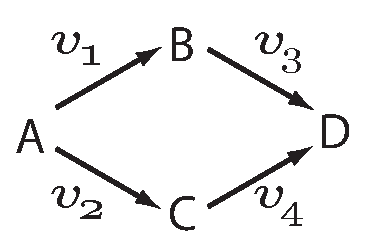
\includegraphics[scale = 0.5]{NetStructExercises1}
\end{figure}
\vspace{-20pt}
(b)
\begin{figure}[H]
\centering
  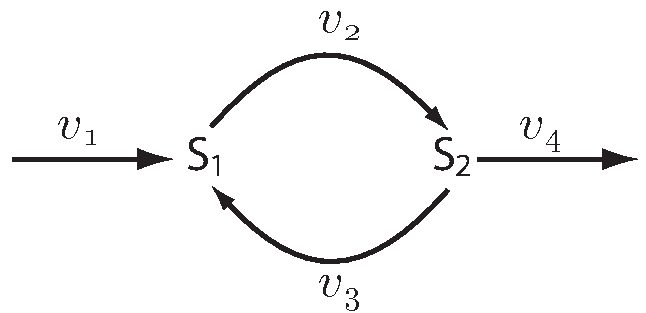
\includegraphics[scale = 0.5]{futileCycle}
\end{figure}
\vspace{-20pt}
(c) \begin{figure}[H]
\centering
  \includegraphics[scale = 0.5]{NetStructExercises2}
\end{figure}
(d) \begin{align*}
\text{A} + \text{X} &\stackrel{v_1}{\longrightarrow} \text{B} + \text{Y} && \text{B} + \text{X} \stackrel{v_2}{\longrightarrow} \text{Y} \\[5pt]
\text{B} &\stackrel{v_3}{\longrightarrow} \text{C} && \text{C} + \text{X} \stackrel{v_4}{\longrightarrow} \text{D} + \text{Y} \\[5pt]
\text{D} + \text{Y} &\stackrel{v_5}{\longrightarrow} \text{X} && \text{X} \stackrel{v_6}{\longrightarrow} \text{Y} \\[5pt]
\text{X} + \text{W} &\stackrel{v_7}{\longrightarrow} 2 \text{Y} && 2 \text{Y} \stackrel{v_8}{\longrightarrow} \text{X} + \text{W} \\[5pt]
\end{align*}
%
\end{question}
\cprotEnv\begin{solution}
\begin{enumerate}[a)]
\item
\begin{equation*}
       \left[ \begin{array}{rrrr}
         -1 & -1 &   0 & 0 \\
          1 & 0  &  -1 & 0 \\
          0 & 1  &   0 & -1 \\
          0 & 0  &   1 & 1 \\
       \end{array} \right]
\end{equation*}

$$\frac{dA}{dt} =  -v_1 - v_2;\ \quad \frac{dB}{dt} = v_1 - v_3;\ \quad \frac{dC}{dt} = v_2 - v_4; \quad \frac{}{} = v_3 + v_4 $$

\item
\begin{equation*}
       \left[ \begin{array}{rrrr}
         1 & -1 &  1 & 0 \\
         0 & 1  &  -1 & -1 \\
       \end{array} \right]
\end{equation*}

$$\frac{dS_1}{dt} = v_1 - v_2 + v_3;\ \quad \frac{dS2}{dt} = v_2 - v_3 - v_4 $$

\item
\begin{equation*}
       \left[ \begin{array}{rrrr}
         -1 & 1  &  0 & 0 \\
          1 & -1 & -1 & 1 \\
          0 & 0  &  1 & -1 \\
       \end{array} \right]
\end{equation*}

$$\frac{dA}{dt} =  -v_1 + v_2;\ \quad \frac{dB}{dt} = v_1 - v_2 - v_3 + v_4;\ \quad \frac{dC}{dt} = v_3 - v_4 $$

\item
\begin{verbatim}
      vo,   v1,  v2,  v2,  v4,  v5,  v6,  v7
A [[  -1,   0,   0,   0,   0,   0,   0,   0],
X  [  -1,  -1,   0,  -1,   1,  -1,  -1,   1],
B  [   1,  -1,  -1,   0,   0,   0,   0,   0],
Y  [   1,   1,   0,   1,  -1,   1,   2,  -2],
C  [   0,   0,   1,  -1,   0,   0,   0,   0],
D  [   0,   0,   0,   1,  -1,   0,   0,   0],
W  [   0,   0,   0,   0,   0,   0,  -1,   1]]

dA/dt = -v0
dX/dt = -v0 - v1 - v3 + v4 - v5 - _6 + v7
dB/dt = v0 - v1 - v2
dY/dt = v0 + v1 + v3 - v4 + v5 + 2.0*v6 - 2.0*v7
dC/dt = v2 - v3
dD/dt = v3 - v4
dW/dt = -v6 + v7
\end{verbatim}
\end{enumerate}

\end{solution}


\begin{question}
For the irreversible enzyme catalyzed reaction, $\text{A} \rightarrow \text{B}$:
\begin{enumerate}[a)]
\item Write out the stoichiometry matrix.

\item Write out the stoichiometry matrix in terms of the elementary reactions that make up the enzyme mechanism.
\end{enumerate}
\end{question}
\begin{solution}
\begin{enumerate}[a)]
\item
\begin{equation*}
       \left[ \begin{array}{rrrr}
         -1 & 1 \\
       \end{array} \right]
\end{equation*}

\item Species order A, E, ES, P
\begin{equation*}
       \left[ \begin{array}{rrrr}
         -1 & 1  &   0  \\
         -1 & 1  &  1  \\
          1 & -1 &   -1  \\
          0 & 0  &   1  \\
       \end{array} \right]
\end{equation*}
\end{enumerate}
\end{solution}


\begin{question}
A gene $G_1$ expresses a protein p$_1$ at a rate $v_1$. p$_1$ forms a tetramer (4 subunits), called p$_1^4$ at a rate
$v_2$. The tetramer negatively regulates a gene $G_2$. p$_1$ degrades at a rate $v_3$. $G_2$ expresses a protein, p$_2$ at a rate $v_9$. p$_2$ is cleaved by an enzyme at a rate $v_4$ to form two protein domains, p$_2^1$ and p$_2^2$. p$_2^1$ degrades at a rate $v_5$. Gene $G_3$ expresses a protein, p$_3$ at a rate $v_6$. p$_3$ binds to p$_2^2$ forming an active complex, p$_4$ at a rate $v_{10}$, which can bind to gene $G_1$ and activate $G_1$. p$_4$ degrades at a rate $v_7$. Finally, p$_2^1$ can form a dead-end complex, p$_5$, with p$_4$ at a rate $v_8$.
\end{question}
\begin{solution}
NA
\end{solution}


\begin{question}
Given the following stoichiometry matrix, write out the corresponding network diagram. Why might this process not fully recover the original
    network from which the stoichiometry matrix was derived?

%\phantom{-}

\begin{equation}
\kbordermatrix{ & v_1 & v_2 & v_3 & v_4 & v_5  \\
\text{A} & -1 &  \phantom{-}0 & -1 &  \phantom{-}0 &  \phantom{-}0  \\
\text{B} &  \phantom{-}1 & -1 &  \phantom{-}0 &  \phantom{-}0 &  \phantom{-}3  \\
\text{C} &  \phantom{-}0 &  \phantom{-}2 & -1 &  \phantom{-}0 &  \phantom{-}0  \\
\text{D} &  \phantom{-}0 &  \phantom{-}0 &  \phantom{-}1 & -1 &  \phantom{-}0  \\
\text{E} &  \phantom{-}0 &  \phantom{-}0 &  \phantom{-}0 &  \phantom{-}1 & -1  \\
\text{F} &  \phantom{-}0 &  \phantom{-}0 &  \phantom{-}0 &  \phantom{-}0 &  \phantom{-}1  \\
\text{G} &  \phantom{-}0 &  \phantom{-}0 &  \phantom{-}0 & -1 &  \phantom{-}0  \\
}
\end{equation}
\end{question}
\begin{solution}
There may be stoichiometry calculations due to the same reactants and products appearing on both sides of a reaction.
\end{solution}


\begin{question}
Derive the mass-balance equations for the following gene regulatory network:

\begin{center}
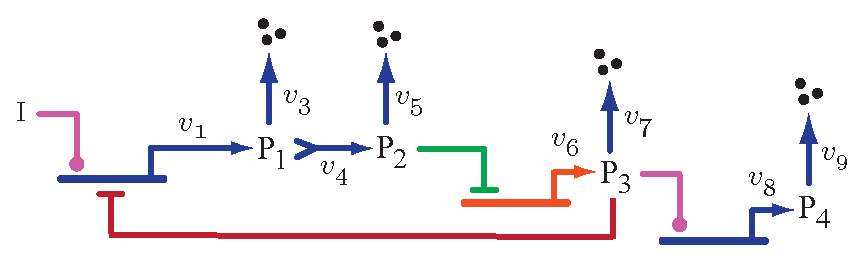
\includegraphics[scale = 0.8]{GeneRegStoichExercise}
\end{center}
\end{question}
\begin{solution}
$$\frac{dP_1}{dt} =  v_1 + v_3 - 2 v_4;\ \quad \frac{dP_2}{dt} = v_4 - v_5 $$

$$\frac{dP_3}{dt} = v_6 - v_7;\ \quad \frac{dP_4}{dt} = v_8 - v_9 $$
\end{solution}



\begin{question}
Why is it better to store a model as a list of reactions rather than a set of differential equations?
\end{question}
\begin{solution}
Storing a model as a list of reactions preserves any stoichiometries that might cancel when converting the scheme to a stoichiometry matrix.
\end{solution}


\ifthenelse{\boolean{myPrintSolutions}}{
\medskip
\begin{center}
{\bf\large Solutions}
\end{center}

\printsolutions[section]
}{}


% ---------------------------------------------------------------------------------------------
\section{Modeling}
% ---------------------------------------------------------------------------------------------

\begin{question}
Which of the following best describes what a model is:
\begin{enumerate}[a)]
\item an attempt to form an exact replica of reality.
\item the truth about the real system.
\item a simplification of the real world.
\end{enumerate}
\end{question}
\begin{solution}
c)
\end{solution}


\begin{question}
State the difference between a deterministic and stochastic model.
\end{question}
\begin{solution}
A deterministic model is one where a given input will always produce the same output. For example, in the equation $y = x^2$, setting $x$ to 2 will always yield the output $4$. A stochastic model is one where the processes described by the model include a random element. This means that repeated runs of a model will yield slightly different outcomes.
\end{solution}


\begin{question}
State the difference between a discrete and continuous model.
\end{question}
\begin{solution}
\begin{enumerate}[a)]
  \item Discrete, stochastic
  \item Although a sand dune is made up of discrete sand particles that appear to move randomly, given the large number of particles and their size, it is more likely one would use a deterministic and continuous model.
  \item Discrete, stochastic.
  \item Continuous, deterministic.
  \item Discrete, deterministic
  \item Discrete model for the individual cells but a continuous model for the growth factors.
\end{enumerate}
\end{solution}



\begin{question}
Suggest what modeling approach you would use for the following systems, i.e.\ continuous or discrete and determisititic or stochastic:
\begin{enumerate}[a)]
\item The spread of a forest fire.
\item Growth and spread of sand dunes.
\item A line of people waiting at cash tills in a store.
\item AM radio electrical circuit.
\item A chess game where both players are computer programs.
\item A tumor where individual cells secrete growth factors.
\end{enumerate}
\end{question}
\begin{solution}
\begin{align*}
\frac{dh_1}{dt} &= (Q_1 - K_1 h_1)/A \\
\frac{dh_2}{dt} &= (K_1 h_1 + K_3 h_3)/A \\
\frac{dh_3}{dt} &= (Q_4 - K_3 h_3)/A
\end{align*}
\end{solution}



\begin{question}
Figure~\ref{fig:ThreeTank} shows three water tanks connected via outflows. Derive the differential equations that describes the rate of change of the heights, $h_1$, $h_2$, and $h_3$. You can assume that the flow rate out of a tank is proportional to the height of water.

\begin{figure}[htb]
\begin{center}
  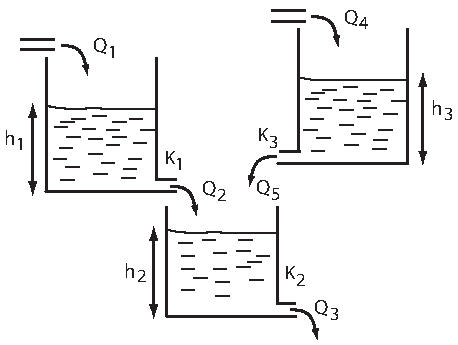
\includegraphics[scale = 1]{ThreeTank}
  \caption{Three tank model.}
  \label{fig:ThreeTank}
\end{center}
\end{figure}
\end{question}
\begin{solution}
\begin{align*}
\frac{dh_1}{dt} &= (Q_1 - K_1 h_1)/A \\
\frac{dh_2}{dt} &= (K_1 h_1 + K_3 h_3)/A \\
\frac{dh_3}{dt} &= (Q_4 - K_3 h_3)/A
\end{align*}
\end{solution}



\begin{question}
State any assumptions or approximations you made in the previous question relating to the water tank model.
\end{question}
\begin{solution}
a) Assumed that the rate of flow out of a tank was proportional tot eh height of water instead of using Torricelli's law. A low water heights a direct proportionality law is approximately true. b) Constant temperature
\end{solution}



\begin{question}
List the three most desirable attributes of a model.
\end{question}
\begin{solution}
Accuracy, predicability and falsifiability.
\end{solution}



\begin{question}
When we ``validate'' a model, which of the following do we most likely mean:
\begin{enumerate}[a)]
\item We show that the model represents the truth about the real system.
\item We increase our confidence in the model's predictive power.
\item We prove that the model is correct.
\end{enumerate}
\end{question}
\begin{solution}
b)
\end{solution}



\begin{question}
Two scientists are arguing about a model, one claims that the model is correct but the other suggests that it is the best so far. Who is making the most reasonable claim and why?
\end{question}
\begin{solution}
The second scientist is making the more reasonable statement that the model is the best so far.
\end{solution}


\begin{question}
Explain the difference between accuracy and predictability of a model.
\end{question}
\begin{solution}
An accurate model is one that can recapitulate the current knowledge about a system.  predictive model is one that can predict new information about a system that is currently not yet known.
\end{solution}


\begin{question}
The authors of a published biochemical model claim that their model has been validated. What do they mean by this?
\end{question}
\begin{solution}
 The authors claiming that their model has been validated means that the model has been shown to correctly predict one or more new experimental data.
\end{solution}


\begin{question}
The author George Box is said to made a statement similar to: ``all models are wrong, but some are useful.''. What does he mean by this?
\end{question}
\begin{solution}
George Box meant that it is not possible to produce a model that is an exact replica of reality (or even desirable), but that simplified models can still generate useful predictions and hence nevertheless useful.
\end{solution}



\begin{question}
The transport of a solute across a membrane is given by the equation $J = P_A (S_{\text{in}} - S_{\text{out}})$. If $P_A$ is expressed in cm $s^{-1}$ and the transport rate in moles cm$^{-2} s^{-1}$, what should the concentrations, $S_{\text{in}}$ and $S_{\text{out}}$ be expressed in?
\end{question}
\begin{solution}
moles cm$^{-3}$
\end{solution}



\begin{question}
What is the difference between a state variable and a boundary variable in a biochemical model?
\end{question}
\begin{solution}
A boundary variable is a quantity of a model that does not change as a result of the action of the model. For a model that uses differential equations, a boundary species does not have a differential equation describing its change. A state variable is a variable that does change as a result of the action of the model.
\end{solution}


\begin{question}
Describe the state variables and types of parameter in the following model of a biochemical pathway:
%
\begin{align*}
\frac{dS_1}{dt} &= k_1 X_o - k_2 S_1 \\[8pt]
\frac{dS_2}{dt} &= k_2 S_1 - (k_3 S_2 - k_4 X_1)
\end{align*}
\end{question}
\begin{solution}
State Variables: $S_1$ and $S_2$. Parameters, $k_1, k_2, k_3$ and $k_4$. Boundary species: $X_o$ and $X_1$.
\end{solution}



\begin{question}
Show that the following functions are nonlinear with respect to $x$:
\begin{enumerate}[a)]
\item $\sin (x)$
\item $e^x$
\item $V_m x/(x + K_m)$
\end{enumerate}
\end{question}
\begin{solution}
\begin{enumerate}
  \item $ \sin(x_1)+\sin(x_2) \neq \sin(x_1 + x_2)) $
  \item $ e^{x_1} + e^{x+2} \neq  e^{x_1 + x_2} $
  \item $ V_m x_1/(K_m + x_1) + V_m x_2/(K_m + x_2) \neq V_m (x_1 + x_2)/(K_m + x_1 + x_2)$
\end{enumerate}
\end{solution}


\begin{question}
Linearize the following functions:
\begin{enumerate}[a)]
\item $4 x^2 + 6 x - 10$ at $x = 1$
\item $V_m x/(x + K_m)$ at $x = 0$ and $x = K_m$
\end{enumerate}
\end{question}
\begin{solution}
\begin{enumerate}
\item Let $f(x)$ be the function to linearise. $\frac{df}{dx} = 8 x + 6 $, therefore at x_o = 1, $y = f(x) + (8 x + 6) (x - 1)$, or $y = 14 x - 14 $

\item Let $f(x)$ be the function to linearise. $\frac{df}{dx} = K_m V_m /(Km + x)^2$. At $x_o = K_m$, $\frac{df}{dx} = V_m/(4 K_m)$, therefore at $x_o = K_m$, $y = f(Km) + V_m/(4 K_m) (x - Km)$. Simplifying this equation yields:
 $ y = V_m/4 +  V_m x (4 K_m) = V_m(K_m + x)/(4 K_m)$
\end{enumerate}
\end{solution}


\begin{question}
In the equation $v = V_m S/(K_m + S)$ where $S$ is expressed in units of mol l$^{-1}$, $V_m$ in mol l$^{-1}$ s$^{-1}$, and the reaction velocity, $v$ in mol l$^{-1}$ s$^{-1}$ what are the units for $K_m$?
\end{question}
\begin{solution}
mol l$^{-l}$
\end{solution}


\begin{question}
In the previous question, if only the units for $S$ are known, what can one say about the units of $K_m$?
\end{question}
\begin{solution}
The units for $K_m$ and $S$ are the same, hence know the units for $S$ automatically gives you the units for $K_m$.
\end{solution}


\ifthenelse{\boolean{myPrintSolutions}}{
\medskip
\begin{center}
{\bf\large Solutions}
\end{center}

\printsolutions[section]
}{}


% ---------------------------------------------------------------------------------------------
\section{Differential Equations}
% ---------------------------------------------------------------------------------------------


\begin{question}
Implement the Euler method in your favorite computer language and use the code to solve the following two problems. Set initial conditions: $S_1 = 10, S_2 = 0$. Set the rate constants to $k_1 = 0.1; k_2 = 0.25$. Investigate the effect of different steps sizes, $h$, on the simulation results.

\medskip
a) $\dS_1/\dt = -k_1 S_1 $ \\

b) $\dS_1/\dt = -k_1 S_1;\ \dS_2/\dt = k_1 S_1 - k_2 S_2$
\end{question}
\cprotEnv\begin{solution}
\begin{verbatim}
import matplotlib.pyplot as plt

# Problem a)

h = 0.1
for k in range (5):
    k1 =0.1; s1 = 10; t = 0
    x = []; y = []
    for i in range (15):
        x.append (t); y.append (s1)
        ds1 = -k1*s1
        s1 = s1 + h*ds1
        t = t + h

    plt.plot (x, y)
    h = h + 4
plt.show()

# Problem b)

h = 0.1
for k in range (5):
    k1 =0.1; k2 = 0.25; s1 = 10; s2 = 0; t = 0
    x = []; y1 = []; y2 = []
    for i in range (15):
        x.append (t);
        y1.append (s1); y2.append (s2)
        ds1 = -k1*s1
        ds2 = k1*s1 - k2*s2
        s1 = s1 + h*ds1
        s2 = s2 + h*ds2
        t = t + h

    plt.plot (x, y1)
    plt.plot (x, y2)
    h = h + 2
\end{verbatim}
\end{solution}


\cprotEnv\begin{question}
The following model shows oscillations in S$_1$ and S$_2$ at a step size of $h = 0.044$ when using the Euler method. Note that species names with a dollar in front are fixed species. By using simulation, show that these oscillations are in fact an artifact.

\begin{verbatim}
   $Xo -> S1; k1*Xo;
    S1 -> S2; k2*S1;
    S2 ->;    k3*S2;

    Xo = 10; S1 = 0; S2 = 0;
    k1 = 23.4; k2 = 45.6; k3 = 12.3;
\end{verbatim}
\end{question}
\cprotEnv\begin{solution}
\begin{verbatim}
h = 0.044
k1 = 23.4; k2 = 45.6; k3 = 12.3
Xo = 10; s1 = 0; s2 = 0
t = 0
x = []; y1 = []; y2 = []
for i in range (15):
    x.append (t);
    y1.append (s1); y2.append (s2)
    ds1 = k1*Xo - k2*s1
    ds2 = k1*s1 - k3*s2
    s1 = s1 + h*ds1
    s2 = s2 + h*ds2
    t = t + h

plt.plot (x, y1)
plt.plot (x, y2)

Set h = 0.001 and the oscillations disappear.
\end{verbatim}
\end{solution}



\begin{question}
Find out what differential equation solvers the Python SciPy Package supports.
\end{question}
\begin{solution}
Python Scipy 1.71 supports the following ODE algorithms: rk23, rk45, rk8, LSODA, Radau, etc.
\end{solution}


\begin{question}
Construct a model of the following system using Tellurium.

{\centering
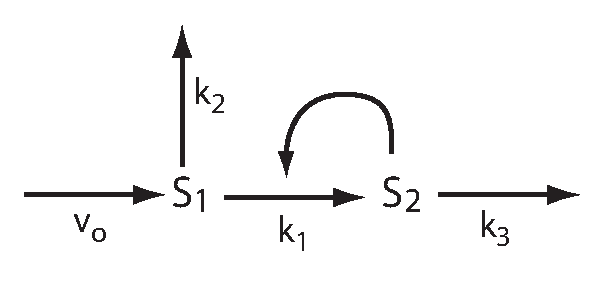
\includegraphics[scale = 0.6]{Heinrich77Model}}

Let the reaction associated with the positive feedback ($k_1$) be governed by the following rate law:
%
$$ k_1 S_1 (1 + c S^q_2) $$

All other reactions are governed by first-order kinetics except the first reaction which has a constant rate of $v_o$. Set the constants to the following values: $v_o = 8; c = 1.0; k_1 = 1; k_2 = 1; k_3 = 5$ and $q = 3$. Study the effect of changing $v_o$ on the dynamics of the system.
\end{question}
\cprotEnv\begin{solution}
\begin{verbatim}
import tellurium as te
import matplotlib.pyplot as plt

r = te.loada("""
     J1:     -> S1;   vo;
     J2:   S1 -> ;    S1*k2;
     J3:   S1 -> S2;  (k1*S1-k_1*S2)*(1+c*S2^q);
     J4:   S2 -> ;    S2*k3;

     S1 = 0; S2 = 0;

    k1 = 1; k2 = 1; k3 = 5;
    q = 3; c = 1; k_1 = 0;  vo = 7;
""")

for i in range (10):
    r.reset()
    m = r.simulate (0, 10, 100)
    plt.plot (m['time'], m['[S1]'])
    r.vo = r.vo + 0.1
plt.show()
\end{verbatim}
\end{solution}


\begin{question}
 Download the model {\tt BIOMD0000000010} from Biomodels (``Kholodenko2000 - Ultrasensitivity and negative feedback bring oscillations in MAPK cascade'') and load it into Tellurium. Run a simulation of the model. Make sure the model is in your current directory. Use {\tt loads} to load a SBML model.
\end{question}
\cprotEnv\begin{solution}
\begin{verbatim}
r = te.loads ('BIOMD0000000010.xml')
m = r.simulate (0, 5000, 1000)
r.plot()
\end{verbatim}
\end{solution}


\begin{question}
Given a system at equilibrium, $A \rightleftharpoons B$, with equilibrium constant, $K_{eq}$, and total mass in the system to be $T = A + B$, show that a change $\delta T$  in the total results in equal proportional changes to A and B.
\end{question}
\begin{solution}
At equilibrium $K_{eq} = B/A$ and $T = A + B$. Therefore $B = T - A$. Solving for B yields: $B = K_{eq} T/(1 + K_{eq})$. If we make a $\delta T$ change in $T$, we can compute $dB/dT$ which equals $dB/dT = K_{eq}/(1 + K_{eq})$. To get the proportional change we multiply by $T$ and divide by $B$ which yields one, i.e a change in T yields a proportional change in $B$ and hence also $A$.
\end{solution}


\ifthenelse{\boolean{myPrintSolutions}}{
\medskip
\begin{center}
{\bf\large Solutions}
\end{center}

\printsolutions[section]
}{}

% ---------------------------------------------------------------------------------------------
\section{Stochastic Models}
% ---------------------------------------------------------------------------------------------


\begin{question}
Define the following terms:

\begin{enumerate}[a)]
  \item $c$
  \item $h$
  \item $h c \delta t$
\end{enumerate}

\end{question}
\begin{solution}
\begin{enumerate}[a)]
 \item $c$ is the average probability that a reactant molecule will react per unit time
 \item $h$ is the number of distinct molecular reactant combinations for a given reaction
 \item $h c \delta t$ is the probability that a reaction will occur in a population of molecules in the next time interval $\delta t$.
\end{enumerate}
\end{solution}


\begin{question}
Given a reaction of the form $X + X \rightarrow $, what is value of $h$
\end{question}
\begin{solution}
$x_a (x_a-1)/2$ where $x_a$ is the number of molecules.
\end{solution}


\begin{question}
The deterministic rate constant for the reaction $2 X \rightarrow $ is equal to 0.5 mM$^{-1}$ s$^{-1}$. If the volume of the compartment in which the reaction takes place is 10 mm$^3$, what is the value for the equivalent stochastic rate constant?
\end{question}
\begin{solution}
We've first convert the units to moles and liters. With that, the value for the deterministic rate constant will be $0.5 \times 10^{-3}$ M s$^{-1}$. The volume, 10 mm$^3$ is converted to $10 \times 10^{-6}$L. To convert we use the expression $2 k/ (N_A V)$ where $N_A$ is Avogadro's number of $6.022 \times 10^{23}$. Hence: $c = 2 \times 0.5 \times 10^{-3} /(6.022 \times 10^{23} \times 10 \times 10^{-6})  = 1.66 \times 10^{-22}$ molecules$^{-1}$ s$^{-1}$.
\end{solution}


\cprotEnv\begin{question}
Given the system:

\begin{verbatim}
    s1 -> s2; k1*s1
    s2 -> s3 + s4; k2*s2
    s4 -> s5; k3*s4

    k1 = 0.1; k2 = 0.34; k3 = 0.02
    s1 = 100
\end{verbatim}

Write a Tellurium script to run a stochastic simulation from time 0 to time 80. Repeat this 10 times and overlay the results on to one graph.
\end{question}
\cprotEnv\begin{solution}
\begin{verbatim}
import tellurium as te

r = te.loada ('''
    s1 -> s2; k1*s1
    s2 -> s3 + s4; k2*s2
    s4 -> s5; k3*s4

    k1 = 0.1; k2 = 0.34; k3 = 0.02
    s1 = 100
''')

for i in range(10):
   m = r.gillespie (0, 80)
   r.plot(m, show=False, alpha=0.8)
   r.reset()

te.show()
\end{verbatim}
\end{solution}


\ifthenelse{\boolean{myPrintSolutions}}{
\medskip
\begin{center}
{\bf\large Solutions}
\end{center}

\printsolutions[section]
}{}


\section{System Behavior}


\begin{question}
Describe the difference between thermodynamic equilibrium and a steady state.
\end{question}
\begin{solution}
Thermodynamic equilibrium is when a system no longer dissipates energy. That is all thermodynamic gradients are at zero, all net fluxes are zero. In steady state, the system dissipates energy at a constant rate (assuming the boundaries of the system are constant).
\end{solution}



\begin{question}
Write out the differential equations for the system $A \rightarrow B \rightarrow C$ where the reactions rates are given by:
%
\begin{align*}
v_1 &= k_1 A - k_2 B \\
v_2 &= k_3 B - k_4 C
\end{align*}

Find the concentrations of A, B, and C when the rates of change are zero: $dA/dt=0, dB/dt=0, dC/dt=0$. Show that this system is at thermodynamic equilibrium when the rates of change are zero.
\end{question}
\begin{solution}
\begin{align*}
\frac{dA}{dt} &= -v_1 \\[5pt]
\frac{dB}{dt} &= v_1 - v_2 \\[5pt]
\frac{dC}{dt} &= v_2
\end{align*}
%
The first thing to realize about this systems is that its closed. This means there is an additional constraint on the system which is that the total mass is fixed, we'll call it $T = A + B + C$. Setting the rates of change to zero and solving for $A, B$ and $C$, and noting that $A = T - B - C$, yields:
%
\begin{align*}
A &= \frac{k_2 k_4 T}{k_1 k_3 + k_1 k_4 + k_2 k_4} \\[5pt]
B &= \frac{k_1 k_4 T}{k_1 k_3 + k_1 k_4 + k_2 k_4} \\[5pt]
C &= \frac{k_1 k_3 T}{k_1 k_3 + k_1 k_4 + k_2 k_4}
\end{align*}

Since the system is closed, the solution to the system, must be at thermodynamic equilibrium. Another way to look at this is to see if the system is dissipating any energy. We can check this by looking at the network fluxes on the first and second steps. For example, substituting the solution for $A$ and $B$ into $v_1$ yields a reaction rate of zero. The same applies to $v_2$.
\end{solution}



\begin{question}
What do we mean by the phrase quasi-equilibrium?
\end{question}
\begin{solution}
Quasi-equilibrium is a phrase that is used to indicate that a subpart of a reaction network is at steady state.
\end{solution}



\begin{question}
Find the mathematical expression that gives the steady state levels of A and B in the following network:

\begin{equation}
\text{X}_o \underset{k_2}{\overset{k_1}{\rightleftharpoons}}
 \text{A} \stackrel{k_3}{\rightarrow} \text{B} \stackrel{k_4}{\rightarrow} \varnothing
\label{model:exSS}
\end{equation}

Assume that $X_o$ is fixed, and that all reactions are governed by simple mass-action kinetics.
\end{question}
\begin{solution}
The differential equations for this system are:

\begin{align*}
\frac{dA}{dt} &= k_1 X_o - k_2 A - k_3 B\\[4pt]
\frac{dB}{dt} &= k_3 A - k_4 B \\
\end{align*}
%
$$ A = \frac{k_1 k_4 X_o}{k_2 k_4 + (k^3)^2} $$
%
$$ B = \frac{k_1 k_3 X_o}{k_2 k_4 + (k_3)^2} $$
\end{solution}




\begin{question}
Consider the following model, use a software tool of your choice to visualize the time evolution for the following system, simulate for 5 time units. At time zero, set $x = 1$ and $y = 2$. Simulate for 30 time units.
%
\begin{align*}
\frac{dx}{dt} &= 0.1 - 0.3 x - 0.4 y \\[5pt]
\frac{dy}{dt} &= 0.5 x + 0.1 y
\end{align*}

Given the model from the previous question, compute the steady state in two ways: 1) Simulating the model for a very long time; 2) Determine algebraically the steady state. Compare the two solutions.
\end{question}
\cprotEnv\begin{solution}
\begin{verbatim}
import tellurium as te
r = te.loada('''
  x' = 0.1 -0.3*x - 0.4*y
  y' = 0.5*x - 0.1*y
  x = 1; y = 2
''')
m = r.simulate (0, 5, 100) # Then change to 30
r.plot()
\end{verbatim}

At $t = 5$, $x = 0.433, y = 0.223$, at $t = 30$, $x = 0.0435, y = 0.217$

Solving the equation algebraically by setting the differential equations to zero yields solutions: $x = 0.0434783$ and $y = 0.217391$.
\end{solution}




\begin{question}
Given the model from the previous question, explore how perturbations in $x$ and $y$ at steady state behave.
\end{question}
\cprotEnv\begin{solution}
\begin{verbatim}
import tellurium as te
r = te.loada('''
  x' = 0.1 -0.3*x - 0.4*y
  y' = 0.5*x - 0.1*y
  x = 0.043478; y = 0.21739

  at time > 10:
      x = x + 1

  at time > 60:
      y = y + 1
''')

m = r.simulate (0, 100, 200)
r.plot()
\end{verbatim}

\end{solution}




\begin{question}
Use a software tool of your choice to visualize the time evolution for the following system, simulate for 5 time units.
%
\begin{align*}
\frac{dx}{dt} &= 2.55 x - 4.4 y \\[5pt]
\frac{dy}{dt} &= 5 x + 2.15 y
\end{align*}
\end{question}
\cprotEnv\begin{solution}
\begin{verbatim}
import tellurium as te
r = te.loada('''
   x' = 2.55*x - 4.4*y
   y'= 5*x + 2.15*y
   x = 1; y = 1
''')

m = r.simulate (0, 5, 200)
r.plot()
\end{verbatim}

The system starts to oscillate uncontrollably.
\end{solution}


\ifthenelse{\boolean{myPrintSolutions}}{
\medskip
\begin{center}
{\bf\large Solutions}
\end{center}

\printsolutions[section]
}{}


% ---------------------------------------------------------------------------------------------
\section{Multicompartment systems}
% ---------------------------------------------------------------------------------------------



\begin{question}
The figure below shows a system of two compartments with volumes $V_1$ and $V_2$. There are three membrane transporters, $P_1, P_2$, and $P_3$ and three cytosolic reactions, $R_1, R_2$, and $R_3$. Write out the differential equations that describe the changes in amounts of $A, B, C$, and $D$. Assume simple facilitated diffusion for the transporters and irreversible first-order kinetics for the reactions. Build a computer model of the system and investigate how the output fluxes at $R_2$ and $R_3$ are influenced by the difference in volume between $V_1$ and $V_2$.

\begin{center}
  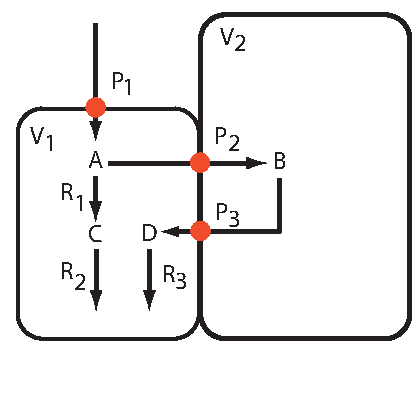
\includegraphics[scale = 0.9]{Compartment1}
\end{center}

    For example, assign reasonable values to all the rate constants in the model, set the two volumes to unity ($V_1 = V_2 = 1$), and compute the two output fluxes. Now increase $V_2$ ten fold while keeping all other parameters the same. What happens to the $R_2$ and $R_3$?

\end{question}
\cprotEnv\begin{solution}
\begin{verbatim}
import tellurium as te
r = te.loada('''
    compartment V1, V2
    var A in V1, C in V1, D in V1
    var B in V2
    ext Out

    P1: -> A; P1_d*(Out - A);
    R1: A -> C; k1*A
    R2: C ->; k2*C

    P2: A -> B; P2_d*(A - B)
    P3: B -> D; P3_d*(B - D)

    R3: D ->; k3*D

    P1_d = 0.1; P2_d = 0.34; P3_d = 0.26
    Out = 1
    k1 = 0.67; k2 = 0.87; k3 = 0.56
    A = 0; B = 0; C = 0; D = 0;

    V2 = 10
''')

m = r.simulate (0, 10, 100)
r.plot()
\end{verbatim}
\end{solution}


\ifthenelse{\boolean{myPrintSolutions}}{
\medskip
\begin{center}
{\bf\large Solutions}
\end{center}

\printsolutions[section]
}{}


% ---------------------------------------------------------------------------------------------
\section{Fitting Models}
% ---------------------------------------------------------------------------------------------


\begin{question}
What are the:
\begin{enumerate}
  \item Chi-square sum of squares
  \item Weighted sum of squares
  \item Reduced chi-square
\end{enumerate}
\end{question}
\begin{solution}
\begin{enumerate}
\item $\sum_{i=1}^N (y_i - f (x_i; p_1\ldots p_m))^2$
\item $\chi^2 \equiv \sum_{i=1}^N \frac{1}{{\sigma_i^2}} \left(y_i - f (x_i; p_1\ldots p_m )\right)^2$
\item $\chi^2_{\text{reduced}} \equiv \frac{1}{N- P}\sum_{i=1}^N \frac{1}{{\sigma_i^2}} \left(y_i - f (x_i; p_1\ldots p_m )\right)^2$
\end{enumerate}
\end{solution}


\begin{question}
Implement a simple gradient descent using Python to find the minimum for $f(x) = 3*x^2 - 4*x + 7$. Use algorithm 4 in Chapter 9 of the textbook
\end{question}
\cprotEnv\begin{solution}
\begin{verbatim}
def fcn (x):
    return 3*x**2 - 4*x + 7

def dfcn (x):
    return 6*x - 4

print ("Gradient Descent")
x = 10; niter = 0
alpha = 0.3

while abs (dfcn (x)) > 1E-4:
    df = dfcn (x)
    x = x - alpha*dfcn (x)
    niter += 1
print (niter, ", x = ", x)
\end{verbatim}
\end{solution}



\begin{question}
Implement a simple gradient descent with a linear search using Python to find the minimum for $f(x) = 3*x^2 - 4*x + 7$. Use algorithm 5 in Chapter 9 of the textbook
\end{question}
\cprotEnv\begin{solution}
\begin{verbatim}
def fcn (x):
    return 3*x**2 - 4*x + 7

def dfcn (x):
    return 6*x - 4

print ("Gradient Descent with line search")
x = 10
alpha = 1; niter = 0

while abs (dfcn (x)) > 1E-4:
#for i in range (20):
    df = dfcn (x)
    alpha = 1;
    while fcn (x - alpha*df) > fcn (x):
      alpha /= 2
    x = x - alpha*df
    niter += 1
print (niter, ", x = ", x)
\end{verbatim}
\end{solution}


\begin{question}
The Levenberg-Marquardt optimization method combines which two simpler methods?
\end{question}
\begin{solution}
It combines a basic gradient descent method with the Guess-Newton method.
\end{solution}


\begin{question}
Name two global optimizer algorithms
\end{question}
\begin{solution}
Differential evolution, simulated annealing, genetic algorithms
\end{solution}


\begin{question}
What two factors does a chi-square test try to distinguish?
\end{question}
\begin{solution}
\begin{enumerate}
\item The normally distributed errors in the experimental data.
\item The choice of model used in the fitting.
\end{enumerate}
\end{solution}


\begin{question}
Students who are new to model fitting are often tempted to fit polynomial functions through data. A typical example is when using Excel to analyse some data where the trend line option gives a variety of fitting functions. A typical plot found in students report is show below:
\begin{center}
\includegraphics[scale=0.5]{overfit.png}
\end{center}
\begin{enumerate}
\item What problem is being highlighted by the fitted plot?
\item Name two statistical test that can be used to help ensure the problem does arise.
\end{enumerate}
\end{question}
\begin{solution}
\begin{enumerate}
\item The student has overfitted the data
\item F-test and AIC values
\end{enumerate}
\end{solution}


\begin{question}
Four models were fitted to the same data. all models appear to fit reasonably well. An AIC value were computed for each model to be 0.8, 15.3, 7.6, and -1.5.

Based on the AIC values which of the four models should we pick for further investigation.
\end{question}
\begin{solution}
We would pick the 4th model because it has the lowest AIC value.
\end{solution}


\begin{question}
The classical approach to estimating confidence limits in fitted parameters is to compute the covariance matrix. What are some of the problems associated with this method?
\end{question}
\begin{solution}
The main problem is that the estimates from the covariance matrix are approximations based on linearising the region around the minimum. This can give a false impression of the actual dimensions of the space around the minimum. In addition it assumes that the experimental noise is normally distritbuted and independent.
\end{solution}


\ifthenelse{\boolean{myPrintSolutions}}{
\medskip
\begin{center}
{\bf\large Solutions}
\end{center}

\printsolutions[section]
}{}


% ---------------------------------------------------------------------------------------------
\section{Steady-State}
% ---------------------------------------------------------------------------------------------


\begin{question}
Consider the following simple branched network:

\begin{center}
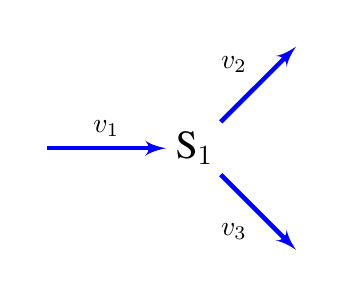
\begin{tikzpicture}[>=latex', node distance=2cm]

  \node (S0) {};
  \node [right of = S0] (S1) {\Large S$_1$};
  \node [above right of = S1] (S2) {};
  \node [below right of = S1] (S3) {};


  \draw [->,ultra thick,blue] (S0) -- node[above, black] {$v_1$} (S1);
  \draw [->,ultra thick,blue] (S1) -- node[above left, black] {$v_2$} (S2);
  \draw [->,ultra thick,blue] (S1) -- node[below left, black] {$v_3$} (S3);
\end{tikzpicture}
\end{center}

where $v_1 = v_o, v_2 = k_1 S_1$ and $v_3 = k_2 S_1$.
\begin{enumerate}[a)]
\item Write the differential equation for $S_1$.
\item Derive the equation that describes the steady state concentration for $S_1$.
\item Derive the equations for the steady state fluxes through $v_1$ and $v_2$.
\item Determine algebraically the scaled sensitivity (See equation~\ref{eqn:scaledSensitivity}) of the steady state concentration of $S_1$ with respect to $v_o$ and $k_1$.
\item Explain why the signs of the sensitivity with respect to $v_o$ and $k_1$ are positive and negative, respectively?
\item Assuming values for $v_o = 1; k_1 = 0.5$ and $k_2 = 2.5$, compute the values for the sensitivities with respect to $k_1$ and $k_2$.
\item What happens to the sensitivity with respect to $k_1$ as $k_1$ increases?
\end{enumerate}

\end{question}
\begin{solution}
\begin{enumerate}[a)]
\item $$ \frac{dS_1}{dt} = v_o - k1 S_1 - k_2 S_1 $$
\item $$ S_1 = \frac{v_o}{k_1 + k_2} $$
\item $$ v_1 = vo, \ v_2 = \frac{k_1 v_o}{k_1 + k_2} $$

$$ \frac{dS_1}{dv_o} \frac{v_o}{S_1} = 1 $$

$$ \frac{dS_1}{dk_1} \frac{k_1}{S_1} = -\frac{k_1}{k_1 + k_2} $$

\item
In $v_o$ increases then this increases the rate of production of $S_1$, therefore $S_1$ rises, hence the sensitivity is positive. With respect to $k_1$, if we increase $k_1$, that causes the rate of $v_2$ increase, which in turn reduces the concentration of $S_1$. Hence the sensitivity is negative.

\item

$$ \frac{dS_1}{dk_1} \frac{k_1}{S_1} = -\frac{k_1}{k_1 + k_2} = -0.5/3 = -0.1666 $$

$$ \frac{dS_1}{dk_2} \frac{k_2}{S_1} = -\frac{k_2}{k_1 + k_2} = 2.5/3 = 0.8333 $$

\item
If $k_1$ is increased then the sensitivity $-\frac{k_1}{k_1 + k_2}$ decreases.
\end{enumerate}
\end{solution}



\begin{question}
Given the equation:

$$ x^2 - a = 0 $$
%
Apply the Newton formula:
%
$$ x_{k+1} = x_k - \frac{f(x_k)}{\partial f/\partial x_k} $$
%
Show that the iterative solution to $x$ is given by:
%
\begin{align}
 x_{k+1} = \frac{1}{2} \left( x_k + \frac{a}{x_k} \right)
 \label{eqn:NRSquareRoot}
\end{align}

\end{question}
\begin{solution}
We apply the algorithm in equation~\eqref{eqn:SimpleNewRaphson} to the problem $x^2 - a = 0$. This leads to:
%
$$ x_{k+1} = x_k - \frac{x^2_k - a}{2 x_k} $$
Simplified, gives:
$$ x_{k+1} = \frac{1}{2} \left( x_k + \frac{a}{x_k} \right) $$
\end{solution}



\begin{question}
Implement the Newton-Raphson algorithm and use it to find {\bf one} solution to the quadratic equation: $4 x^2 + 6 x - 8 = 0$.
\end{question}
\begin{solution}
Software project. The solutions to $4 x^2 + 6 x - 8 = 0$ are $1/4 (-3-sqrt{41})$ and $1/4 (-3+sqrt{41})$ or 0.851 and -2.35
\end{solution}



\begin{question}
By changing the initial starting point of the Newton-Raphson algorithm, find the second solution to the quadratic equation from the previous question.
\end{question}
\begin{solution}
Programming project.
\end{solution}



\begin{question}
Using Tellurium, find the steady state for the following model:

{\tt Xo -> S1; k1*Xo; S1 -> X1; k2*S1; S1 -> X2; k3*S1;}

Assume that {\tt Xo, X1} and {\tt X2} have fixed concentrations with values $Xo=1; X_1 = 0; X_2 = 0$ and rate constants $k_1 = 0.1; k_2 = 0.35; k_3 = 0.45$. Compute the steady state concentration of {\tt S1}.
\end{question}
\cprotEnv\begin{solution}
\begin{verbatim}
r = te.loada ('''
   $Xo -> S1; k1*Xo
   S1 -> $X1; k2*S1
   S1 -> $X2; k3*S1
   k1 = 0.1; k2 = 0.35; k3 = 0.45
   Xo = 1
  ''')

r.steadyState()
print (r.S1)
\end{verbatim}
\end{solution}



\begin{question}
Write a Tellurium script to perturb the value of {\tt Xo} in the above model. Apply the perturbation as a square pulse; that is, the concentration of {\tt Xo} rises, stays constant, then falls back to its original value. Make sure the system is at steady state before you apply the perturbation.
\end{question}
\cprotEnv\begin{solution}
\begin{verbatim}
r = te.loada ('''
   $Xo -> S1; k1*Xo
   S1 -> $X1; k2*S1
   S1 -> $X2; k3*S1
   k1 = 0.1; k2 = 0.35; k3 = 0.45
   Xo = 1

   at time > 30:
       Xo = Xo + 1
   at time > 50:
       Xo = Xo - 1
''')

m = r.simulate (0, 100, 200)
r.plot()
\end{verbatim}
\end{solution}



\begin{question}
Explain what is meant by a stable and unstable steady state.
\end{question}
\begin{solution}
A stable steady state is one where a perturbed species relaxes back to the ordinal steady state. If the steady state is unstable, and perturbation will not recover and will evolve to a new value.
\end{solution}




\begin{question}
The steady state of a given pathway is stable. Explain the effect in general terms on the steady state if:

a) A bolus of floating species is injected into the pathway.

b) A permanent change is applied to a kinetic constant.
\end{question}
\begin{solution}
\begin{enumerate}[a)]
\item The floating species will initially rise but will in time fall back to it original steady state value.
\item The rate constant is increased, this will result in the steady state change to a new state.
\end{enumerate}
\end{solution}


\begin{question}
Why are scaled sensitivities sometimes more advantageous that unscaled sensitivities?
\end{question}
\begin{solution}
Scaled sensitivities are more useful because they are unit less and can be approximated as a ration of percentage changes. Such changes are more easily measured than absolute values.
\end{solution}


\begin{question}
Construct a simple linear pathway with four enzymes as shown below:
%
\begin{center}
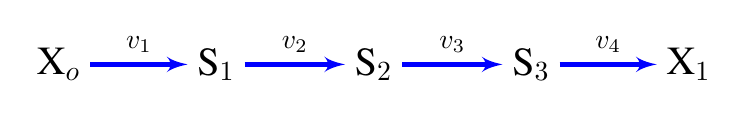
\begin{tikzpicture}[>=latex', node distance=2cm]

  \node (S1) {\Large X$_o$};
  \node [right of = S1] (S2) {\Large S$_1$};
  \node [right of = S2] (S3) {\Large S$_2$};
  \node [right of = S3] (S4) {\Large S$_3$};
  \node [right of = S4] (S5) {\Large X$_1$};

  \draw [->,ultra thick,blue] (S1) -- node[above, black] {$v_1$} (S2);
  \draw [->,ultra thick,blue] (S2) -- node[above, black] {$v_2$} (S3);
  \draw [->,ultra thick,blue] (S3) -- node[above, black] {$v_3$} (S4);
  \draw [->,ultra thick,blue] (S4) -- node[above, black] {$v_4$} (S5);

\end{tikzpicture}
\end{center}

Assume that the edge metabolites, X$_o$ and X$_1$, are fixed. Assign reversible Michaelis-Menten kinetics to each step and arbitrary values to the kinetics constants.  Assign a modest value to the boundary metabolite, X$_o$, of 10 mM. Compute the steady state for your pathway. If the software fails to find a steady state, adjust the parameters. Once you have the steady state, use the model to compute the sensitivity of the steady state flux with respect to each of the enzyme maximal activities. You can compute each sensitivity by perturbing each maximal activity and observing what this does to the steady state flux.

How might you use the flux sensitivities in a practical application? Compute the sum of the four sensitivities, what value do you get? Can you make a statement about the sum?
\end{question}
\begin{solution}
Programming project
\end{solution}


\ifthenelse{\boolean{myPrintSolutions}}{
\medskip
\begin{center}
{\bf\large Solutions}
\end{center}

\printsolutions[section]
}{}


% ---------------------------------------------------------------------------------------------
\section{Stability}
% ---------------------------------------------------------------------------------------------




\begin{question}
Determine the Jacobian matrix for the following system that describes a branched pathway:
%
\begin{align*}
\frac{dS_1}{dt} &= v_o - k_1 S_1 - k_2 S_1 \\[5pt]
\frac{dS_2}{dt} &= k_2 S_1 - k_3 S_2 - k_4 S_2
\end{align*}
\end{question}
\begin{solution}
$$
\begin{bmatrix}\\[-8pt]
-k_1 & -k_2 \\[7pt]
k_2 & -(k_3 + k_4) \\[7pt]
\end{bmatrix}
$$
\end{solution}


\begin{question}
Determine the Jacobian matrix for the following two systems:
%
\begin{align*}
\text{a)}\ \frac{dx}{dt} &= x^2 - y^2 \quad \frac{dy}{dt} = x (1 - y) \\[10pt]
\text{b)}\ \frac{dx}{dt} &= y - x y \quad \frac{dy}{dt} = x y
\end{align*}
\end{question}
\begin{solution}
\begin{enumerate}[a)]
\item
$$
\begin{bmatrix}\\[-8pt]
2x & -2y \\[7pt]
1-y & -x \\[7pt]
\end{bmatrix}
$$
\item
$$
\begin{bmatrix}\\[-8pt]
-y & 1-x \\[7pt]
y & x \\[7pt]
\end{bmatrix}
$$
\end{enumerate}
\end{solution}


\begin{question}
Determine the Jacobian in terms of the unscaled elasticities and stoichiometry matrix for the following three systems. Assume all reactions are product insensitive, $X_i$ species are fixed, and in c) $S_3$ regulates the first step, $S_1 \rightarrow S_2$.


\begin{align*}
\text{a)}\ X_o &\rightarrow S_1;\ S_1 \rightarrow S_2;\ S_2 \rightarrow S_3; S_3 \rightarrow X_1\\[5pt]
\text{b)}\ X_o &\rightarrow S_1;\ S_1 \rightarrow S_2;\ S_2 \rightarrow S_1;\ S_2 \rightarrow X_1\\[5pt]
\text{c)}\ S_1 &\rightarrow S_2;\ S_2 \rightarrow S_3
\end{align*}

\end{question}
\cprotEnv\begin{solution}
Stable
\begin{verbatim}
import telluirum as te
r = te.loada ('''
    $Xo -> S1;  Vm1*Xo/(Km1 + Xo + S1/K1);
    S1 -> S2; Vm2*S1/(Km2 + S1 + S2/K2)
    S2 -> $X1; Vm3*S2/(Km3 + S2)

    // Set up the model initial conditions
    Xo = 1; X1 = 0
    Vm1 = 1.5; Vm2 = 2.3; Vm3 = 1.9
    Km1 = 0.5; Km2 = 0.6; Km3 = 0.45
    K1 = 0.1; K2 = 0.2
''')

# Evaluation of the steady state
print (r.getSteadyStateValues())
# print the eigenvalues of the full Jacobian matrix
print (r.getFullEigenValues())

[0.23769588 0.11506555]
[-1.5956469 +0.j -4.80299766+0.j]
\end{verbatim}

Both eigenvalues have negative real parts hence the system is stable.
\end{solution}



\begin{question}
Show that the following system is stable to perturbations in S$_1$ and S$_2$ by computing the eigenvalues at steady state (See Listing~\ref{jarnac:chap:eigenvaluestability}):
%
$$ \text{X}_o \stackrel{v_1}{\rightarrow} \text{S}_1 \stackrel{v_2}{\rightarrow} \text{S}_2 \stackrel{v_3}{\rightarrow} \text{X}_1 $$
%
The three rate laws are given by:
%
\begin{align*}
v_1 &= \frac{V_{m_1} X_o}{Km_1 + X_o + S_1/K_1} \\[5pt]
v_2 &= \frac{V_{m_2} S_1}{Km_2 + S_1 + S_2/K_2} \\[5pt]
v_3 &= \frac{V_{m_3} S_2}{Km_3 + S_2} \\[5pt]
\end{align*}
%
Assign the following values to the parameters: $X_o = 1; X_1 = 0; V_{m_1} = 1.5; V_{m_2} = 2.3; V_{m_3} = 1.9; K_{m_1} = 0.5$; $K_{m_2} = 0.6; K_{m_3} = 0.45; K_1 = 0.1; K_2 = 0.2$.
\end{question}
\begin{solution}
\begin{enumerate}[a)]
\item $$
\begin{bmatrix}\\[-8pt]
-\varepsilon^2_1 & 0 & 0 \\[7pt]
\varepsilon^2_1 & -\varepsilon^3_2 & 0 \\[7pt]
0 & \varepsilon^3_2 & -\varepsilon^4_3  \\
\end{bmatrix}
$$
\item
$$
\begin{bmatrix}\\[-8pt]
-\varepsilon^2_1 & \varepsilon^3_2  \\[7pt]
\varepsilon^2_1 & -\varepsilon^3_2 -\varepsilon^4_2 \\
\end{bmatrix}
$$
\item
$$
\begin{bmatrix}\\[-8pt]
-\varepsilon^1_1 & 0 & -\varepsilon^1_3 \\[7pt]
\varepsilon^1_1 & -\varepsilon^2_2 & 0 \\[7pt]
0 & \varepsilon^2_2 & 0 \\
\end{bmatrix}
$$
\end{enumerate}
\end{solution}



\begin{question}
Given the Jacobian matrix you evaluated in first question of this section, do you think the system will stable or unstable? Hint: The eigenvalues of a triangular matrix are equal to the elements of the main diagonal.
\end{question}
\begin{solution}
The Jacobian has a triangular form, hence the eigenvalues are the values on the main diagonal, which in this case are $-k_1$ and $-(k_3+k_4)$. Since rate constants are positive, the eigenvalues must be negative. Hence the system is stable.
\end{solution}


\cprotEnv\begin{question}
Show that the following system is unstable. What kind of unstable dynamics does it have?

\begin{verbatim}
import tellurium as te

r = te.loada ('''
    J0: $X0 -> S1; VM1*(X0-S1/Keq1)/(1+X0+S1+pow(S4,h));
    J1: S1 -> S2; (10*S1-2*S2)/(1+S1+S2);
    J2: S2 -> S3; (10*S2-2*S3)/(1+S2+S3);
    J3: S3 -> S4; (10*S3-2*S4)/(1+S3+S4);
    J4: S4 -> $X1; Vm4*S4/(KS4+S4);

    X0 = 10;       X1 = 0;
    S1 = 0.973182; S2 = 1.15274;
    S3 = 1.22721;  S4 = 1.5635;
    VM1 = 10;      Keq1 = 10;
    h = 4;        Vm4 = 2.5;
    KS4 = 0.5;
''')
\end{verbatim}
\end{question}
\cprotEnv\begin{solution}

Using the commands:
\begin{verbatim}
# Evaluation of the steady state
print (r.getSteadyStateValues())
# print the eigenvalues of the full Jacobian matrix
print (r.getFullEigenValues())
\end{verbatim}
to compute the eigenvalues for the system. Running this code yields:
\begin{verbatim}
-0.24875048+1.04230509j, -0.24875048-1.04230509j,
 -4.35227266+0.j -,5.35539319+0.j
\end{verbatim}
This includes two eigenvalues with negative real parts and a conjugate pair also with negative real parts. This corresponds to a stable spiral. that is a damped oscillation.
\end{solution}



\cprotEnv\begin{question}
Show that the following system is unstable. What kind of unstable dynamics does it have?

\begin{verbatim}
import tellurium as te

r = te.loada ('''
    J0:  $src -> X;    k1*S;
    J1:  X -> R;       (kop + ko*EP)*X;
    J2:  R -> $waste;  k2*R;
    J3:  E -> EP;      Vmax_1*R*E/(Km_1 + E);
    J4:  EP -> E;      Vmax_2*EP/(Km_2 + EP);

    src = 0;      kop = 0.01;
    ko =  0.4;    k1 = 1;
    k2 = 1;       R = 1;
    EP = 1;       S = 0.2;
    Km_1 = 0.05;  Km_2 = 0.05;
    Vmax_2 = 0.3; Vmax_1 = 1;
    KS4 = 0.5;
''')

result = r.simulate(0, 500, 1000)
r.plot()
\end{verbatim}
\end{question}
\begin{solution}
The system shows sustained oscillations with an alternation of rapid and slow dynamics.
\end{solution}


\ifthenelse{\boolean{myPrintSolutions}}{
\medskip
\begin{center}
{\bf\large Solutions}
\end{center}

\printsolutions[section]
}{}


% ---------------------------------------------------------------------------------------------
\section{Feedforward Networks}
% ---------------------------------------------------------------------------------------------


\begin{question}
Study the behavior of an Incoherent Type I FFL by using a competitive model for the activator/repression step. In a competitive model both the repressor and activator bind to the same operator site.
\end{question}
\begin{solution}
The competitive model (taken from Enzyme Kinetics for Systems Biology) is of the form:

$$ v = V_f \frac{K_1 A^n}{1 + K_1 A^n + K_2 A^B} $$

Use the script shown in listing~\ref{jarnac:IncoherentTypeIPulse}.

Study the effect of pulses and step inputs on the dynamics of the feed forward network
\end{solution}


\ifthenelse{\boolean{myPrintSolutions}}{
\medskip
\begin{center}
{\bf\large Solutions}
\end{center}

\printsolutions[section]
}{}


% ---------------------------------------------------------------------------------------------
\section{Behavior of Stochastic Models}
% ---------------------------------------------------------------------------------------------



\cprotEnv\begin{question}
The following modified model is taken from the work of Ribeiro and Lloyd-Price~\cite{ribeiro2007}. Run a simulation of the model using the given parameters. Explain why this model shows bimodal behavior.

\begin{verbatim}
import tellurium as te

r = te.loada ('''
    ProA -> A + ProA; g*ProA;
    ProB -> B + ProB; g*ProB;
    A + ProB -> ProBA; a0*A*ProB;
    B + ProA -> ProAB; a0*B*ProA;
    ProBA -> ProB + A; a1*ProBA;
    ProAB -> ProA + B; a1*ProAB;
    A -> $w; d*A;
    B -> $w; d*B;

    g = 0.2;   d = 0.01;
    a0= 0.3;   a1 = 0.05;
    A = 0;     B = 0;
    ProA = 1;  ProB = 1;
''')

r.setSeed(random.randint (1, 1000000))
result = r.gillespie(0, 2000000, ["Time", "A"]);
r.plot()
\end{verbatim}
\end{question}
\begin{solution}
The model has two steady states, high A, low B and low A, high B. This is caused by competition of A and B for ProB and ProA. ProA and ProB are present in only single copies. For example, once A bind with ProB to form the complex ProBA, the production of B stops. This prevents B from sequestering ProA so that A starts to increase, reaching a high state for A (the level is governed by the decay rate of A) with a very low or zero level for B. By chance, the complex ProBA can decay in A and ProB. This gives ProB the chance to start making B. With B rising it is possible for B to sequester ProA, shutting down production of A. If this lasts long enough A will decay and B will rise switching the system to the other state with a low A and high B. The system can therefore switch back and forth. Switching from one state to another is random and depends on the decay of the complex ProA or ProB. If the levels of ProA and ProB are increased, there is less chance of removing all copies of each in order to switch the system. At molecule numbers of 100 for ProA and ProB, the system is quite stable.
\end{solution}



\begin{question}
The following model should be simulated as a deterministic model (i.e.\ using ODEs) and
as a stochastic model.

\begin{figure}[htb]
  \begin{center}
  \includegraphics[scale=0.2]{Howard.pdf}
  \end{center}
  \caption{Reaction Scheme: Xo, X1, and X2 are boundary species. Be very careful that you replicate this model exactly as given.
  Assume all reactions are simple irreversible mass-action. Parameter values are
  as follows: $k_1 = 0.1; k_2 = 0.1; k_3 = 0.01; k_4 = 0.05; k_5 = 10.1; Xo = 10; X_1 = 0; X_2 = 1$. Note that the $k_2$ reaction is {\tt S1 + S2 -> S3 + 2 S3}}
\end{figure}

\begin{enumerate}[a)]
\item Enter the model into Tellurium and run a deterministic simulation.
Show the graphs for $S_1$, $S_2$, and $S_3$ over a time period of 800
time units.

\item Next run the same model as a stochastic model (use gillespie() instead of simulate())
Use the same values for the rate constants and initial conditions.
Plot $S_1$ and $S_3$ on one graph and $S_2$ on another graph. As with the deterministic model, simulate for 800 time units.

\item Observe the significant difference between the deterministic and
stochastic simulations. Why is this the case? Explain why the dynamics of the stochastic
simulation are so different considering the number of
molecules involved and the kind of reactions in the models.

\item Given your answer in (c), provide one situation where you think it is important to use a
stochastic model rather than a deterministic one.
\end{enumerate}
\end{question}
\cprotEnv\begin{solution}
The script to run the deterministic and stochastic model are given below.
\begin{verbatim}
import tellurium as te
import matplotlib.pyplot as plt

r = te.loada ('''
       $Xo -> S1; k1*Xo
       S1 + S2 -> 2 S2 + S3; k2*S1*S2
       S3 -> $X1; k3*S3;
       $X2 -> S2; k4*X2;
       S2 -> $X1; k5*S2

       k1 = 0.1; k2 = 0.1; k3 = 0.01; k4 = 0.05; k5 = 10.1;
       Xo = 10; X2 = 1

''')

m = r.simulate (0, 800, 100)
plt.figure(figsize=(10,3))
plt.subplot(1, 2, 1)
plt.plot (m['time'], m['[S1]'])
plt.plot (m['time'], m['[S3]'])
plt.subplot(1, 2, 2)
plt.plot (m['time'], m['[S2]'])
plt.show()

r.reset()
m = r.gillespie (0, 800)
plt.figure(figsize=(10,3))
plt.subplot(1, 2, 1)
plt.plot (m['time'], m['[S1]'])
plt.plot (m['time'], m['[S3]'])
plt.subplot(1, 2, 2)
plt.plot (m['time'], m['[S2]'])
plt.show()
\end{verbatim}
Clearly the two cases are quite different. The main difference is how $X_2$ enters the model. In the deterministic case a value of $X_2 = 1$, generates a fixed rate of 0.05. This causes $S_2$ to slowly increase. The reaction $k_2$ is autocatalytic and once some $S_2$ is made the positive feedback of the autocatalytic reaction results in a significant and rapid rise in $S_2$. Eventually the system reaches a steady state as a result of $k_5$.

In the stochastic case a value of one for $X_2$ represents a single molecule. The rate of production of $S_2$ is therefore highly stochastic. If an event at $k_4$ cases the production of one molecule of $S_2$, two things can happen, $S_2$ can decay via $k_5$ and nothing more happens until $k_4$ fires again. However if reaction $k_2$ fires before $k_5$, then it is possible for the autocatalytic cycle to start up resulting in more $S_2$. This can cause $S_2$ to rise rapidly. However, the autocatalytic cycle is depending on $S_1$ and $S_1$ is produced via $X_o$, another reaction that will only generate a single molecule of $S_1$ per firing (but with a higher frequency since $X_o = 10$). It is possible therefore that if $k_1$ doesn't fire for some time, $S_1$ could decay to zero, resulting in the autocatalytic cycle shutting off. This might give sufficient time for $k_5$ to eliminate $S_2$ and the cycle can begin again. This results is a cycle of boom and busts in $S_1$ and $S_3$. Instead of reaching a steady-state, the system appears to oscillate.

In conclusion, it is important to use a stochastic model when ever there are single events (like $k_4$) that can have a huge influence on the future state of the system particularly if a single event can be amplified.
\end{solution}

%
%\begin{question}
%Expand the simple gene expression model in Figure~\ref{fig:BurstingModel} to include transcription and translation. Develop a stochastic model of the expanded system. Investigate whether the translation machinery, which is present in higher concentration, can act as a buffer to the mRNA bursting.
%\end{question}
%\begin{solution}
%No solution yet
%\end{solution}

\end{document}

